\documentclass{beamer}

\usepackage{amsmath}
\usepackage{amssymb}
\usepackage{amsthm}
\usepackage{mathtools}
\usepackage[UKenglish]{babel}
\usepackage{enumerate}
\usepackage{graphicx}
\usepackage{braket}
\usepackage{esint}
\usepackage{float}
\usepackage{tabularx}
\usepackage{array}
\usepackage{subcaption}
\usepackage{hyperref}
\usepackage{xcolor}
\hypersetup{colorlinks=false, bookmarks=true}

\usetheme{Madrid}
\usecolortheme{seahorse}
\usefonttheme{professionalfonts}
\useinnertheme{circles}

\AtBeginSection[]
{
  \begin{frame}
    \frametitle{Table of Contents}
    \tableofcontents[currentsection]
  \end{frame}
}

\setbeamertemplate{caption}[numbered]

\title[QCNN State Preparation]{A QCNN for Quantum State Preparation}
\subtitle{Carnegie Vacation Scholarship}
\author[David Amorim]{David Amorim}
\institute[]{}
\date[14/08/2024]{Week 6 \\(05/08/2024 - 14/08/2024)}

\begin{document}

\frame{\titlepage}

\begin{frame}
\begin{exampleblock}{Erratum}
The slides for the previous weeks showed the wrong placement of the absolute signs in the definition of SAM. The definition should read:
\begin{equation}
\text{SAM}(\ket{x}, \ket{y}) = 1 - \sum_k |x_k| | y_k |.  
\end{equation}
This has now been corrected. Equivalently for WIM. 
\end{exampleblock}
\end{frame}

\begin{frame}
\frametitle{Aims for the Week}
The following aims were set at the last meeting (05/08/2024):

\begin{alertblock}{Generalise Input States}
When training in superposition, feed in a wider range of input states to ensure the network learns as intended. 
\end{alertblock}

\begin{alertblock}{Work on Code and Documentation}
Continue re-structuring and re-documenting the code to ensure a smooth handover. 
\end{alertblock}

TRY AND DO SOME BARREN PLATEAU ???

\end{frame}

\section{Generalised Input States}

\begin{frame}
\frametitle{Generalised Input States}

\begin{itemize}
\item When training in superposition, the QCNN now takes the input state 
\begin{equation}
\ket{\psi}_\text{{in}} =\sum^{2^n-1}_{j=0} c_j \ket{j} 
\end{equation}
where the \alert{coefficients} $c_j \sim \frac{1}{\sqrt{2^n}}$ are \alert{randomly sampled} each epoch
\item The \alert{range} of the random sampling is controlled by a \alert{hyper-parameter $\delta$},  $0 \leq \delta \leq 1$ 
\item For instance,  $\delta=0$ gives $c_j = \frac{1}{\sqrt{2^n}}$ while $\delta =1$ gives $c_j \in (0,1)$
\item This generalisation should ensure that the network learns the operation $\ket{j} \ket{0} \mapsto \ket{j} \ket{\Psi'(j)}$ as opposed to just learning how to produce a particular fixed state
\end{itemize}
\end{frame}

\begin{frame}
\frametitle{Results}
Amplitudes after applying $\tilde{Q}$ with $\Psi(f) \sim f^2$ and the input register in initial state $\hat{H} \ket{0}$ ($L=\boldsymbol{9}$, $m=3$, SAM, 600 epochs):
\begin{columns}
\begin{column}{0.5\textwidth}
\begin{figure}
\centering
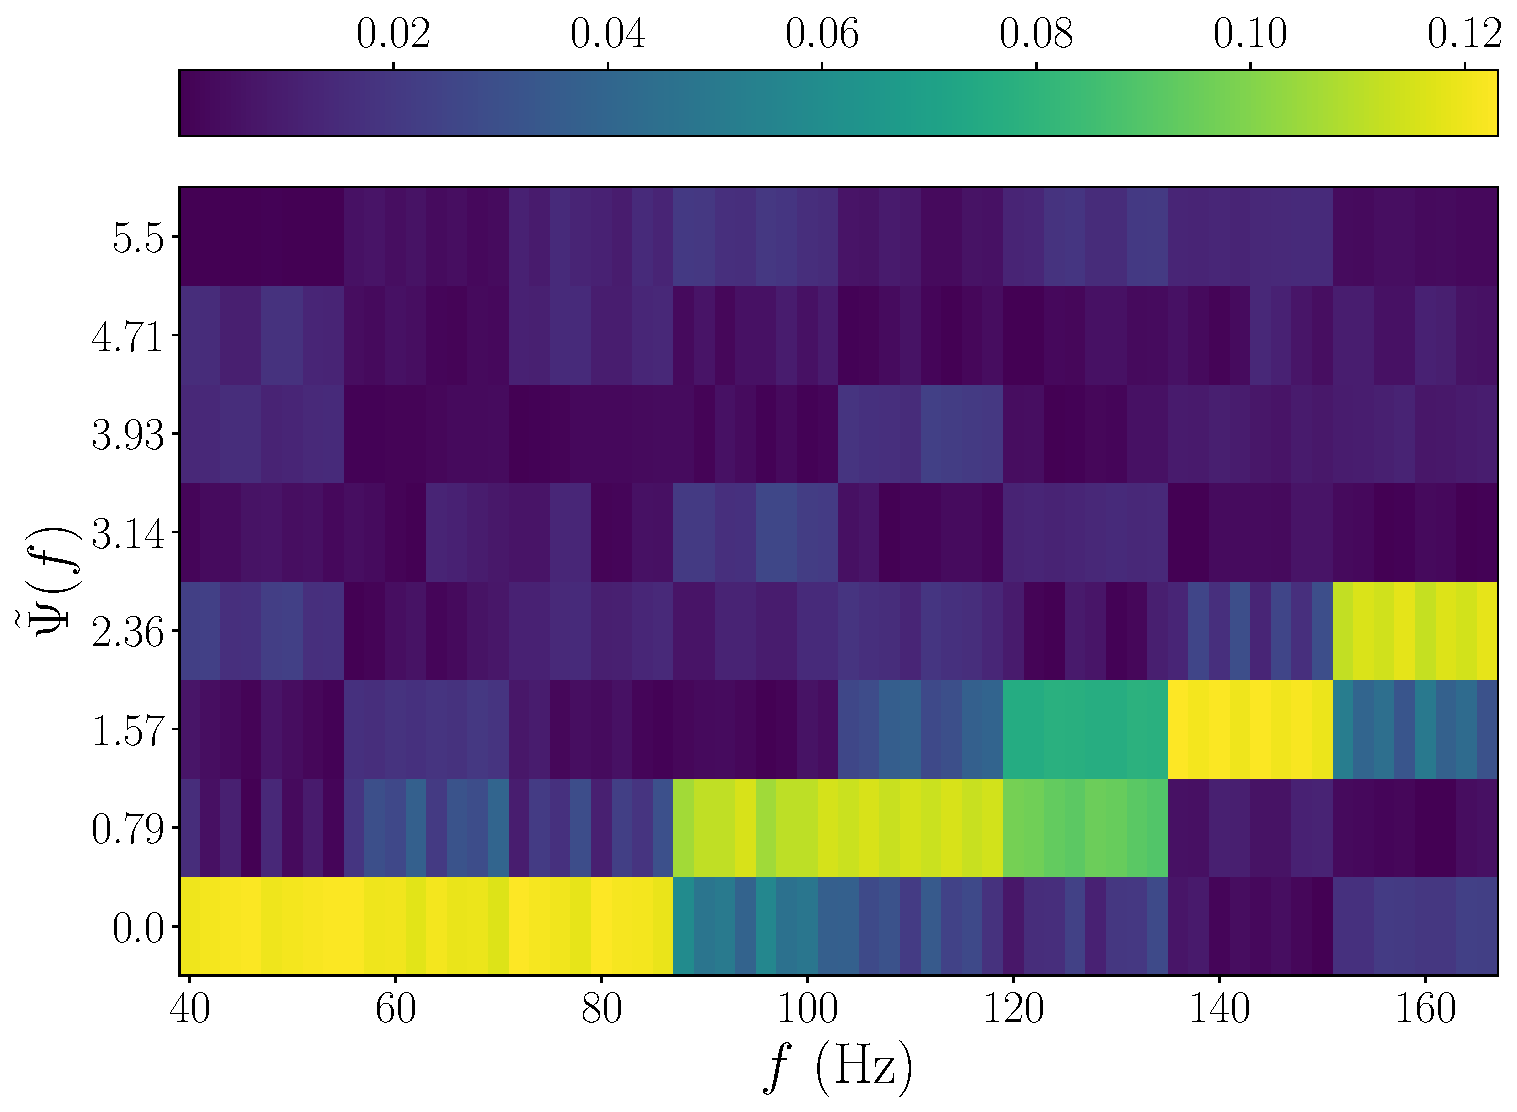
\includegraphics[width=\textwidth]{im/Q_amp_quadratic_0.0_H.pdf}
\caption{$\delta =0$}
\end{figure}
\end{column}
\begin{column}{0.5\textwidth}
\begin{figure}
\centering
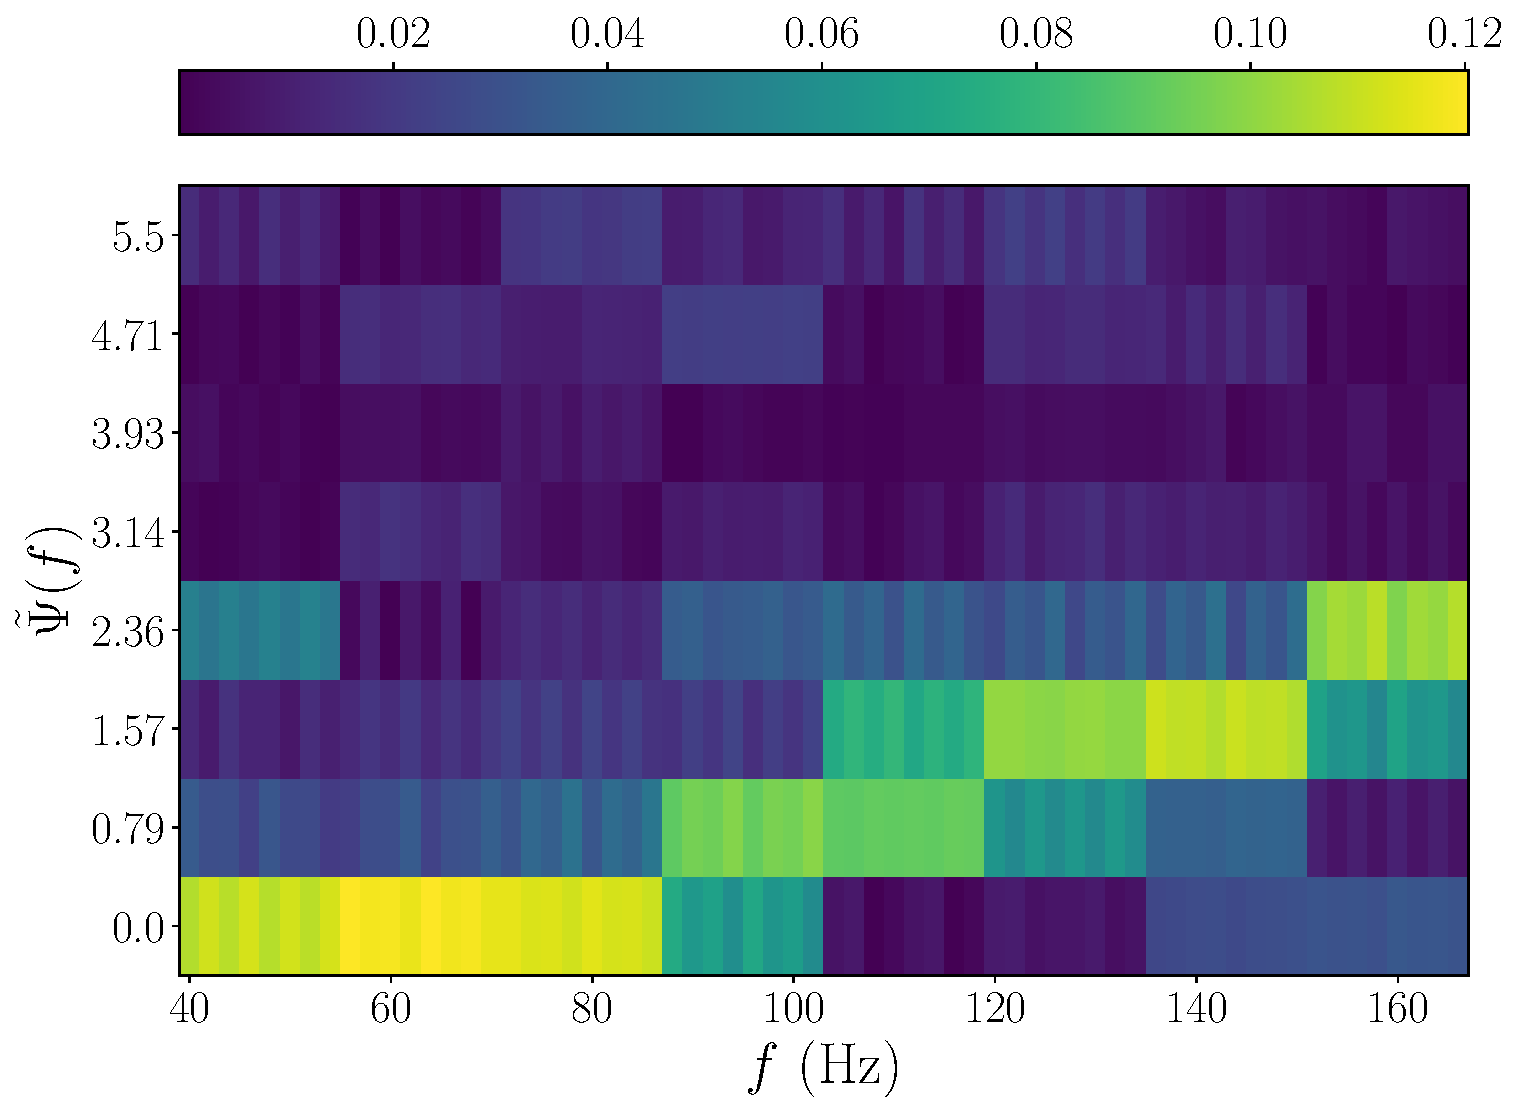
\includegraphics[width=\textwidth]{im/Q_amp_quadratic_0.2_H.pdf}
\caption{$\delta =0.2$}
\end{figure} 
\end{column}
\end{columns}
\end{frame}

\begin{frame}
\frametitle{Results}
Amplitudes after applying $\tilde{Q}$ with $\Psi(f) \sim f^2$ and the input register in initial state $\hat{H} \ket{0}$ ($L=\boldsymbol{9}$, $m=3$, SAM, 600 epochs):
\begin{columns}
\begin{column}{0.5\textwidth}
\begin{figure}
\centering
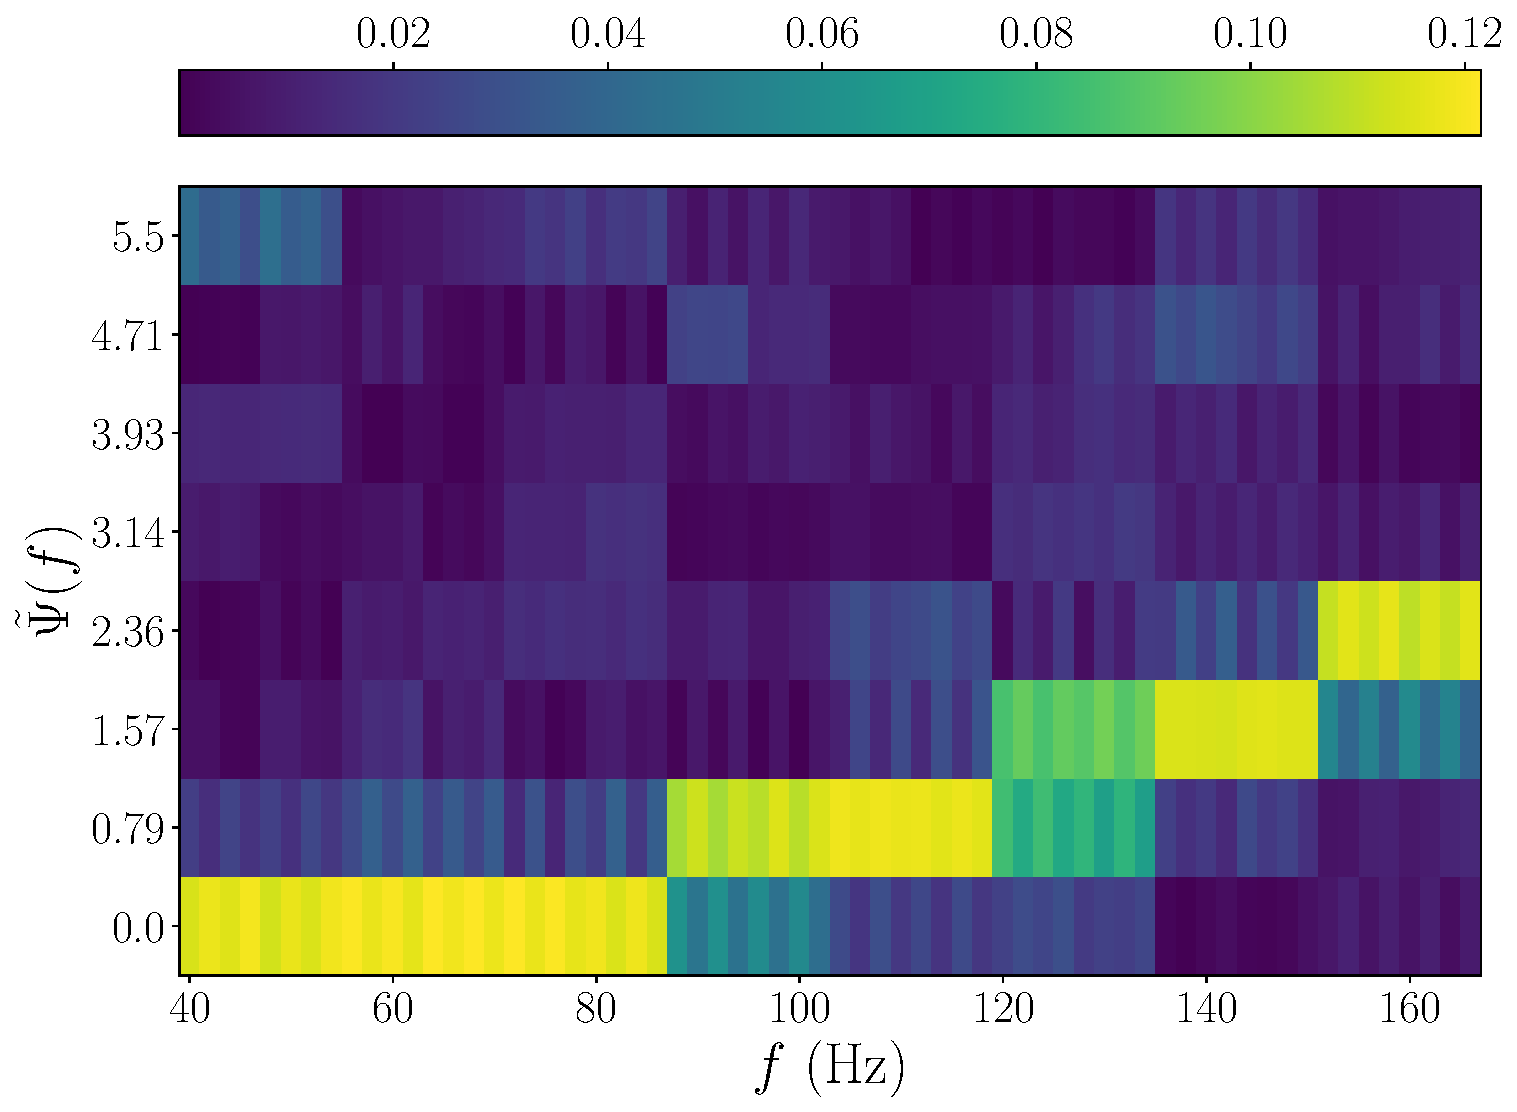
\includegraphics[width=\textwidth]{im/Q_amp_quadratic_0.4_H.pdf}
\caption{$\delta =0.4$}
\end{figure}
\end{column}
\begin{column}{0.5\textwidth}
\begin{figure}
\centering
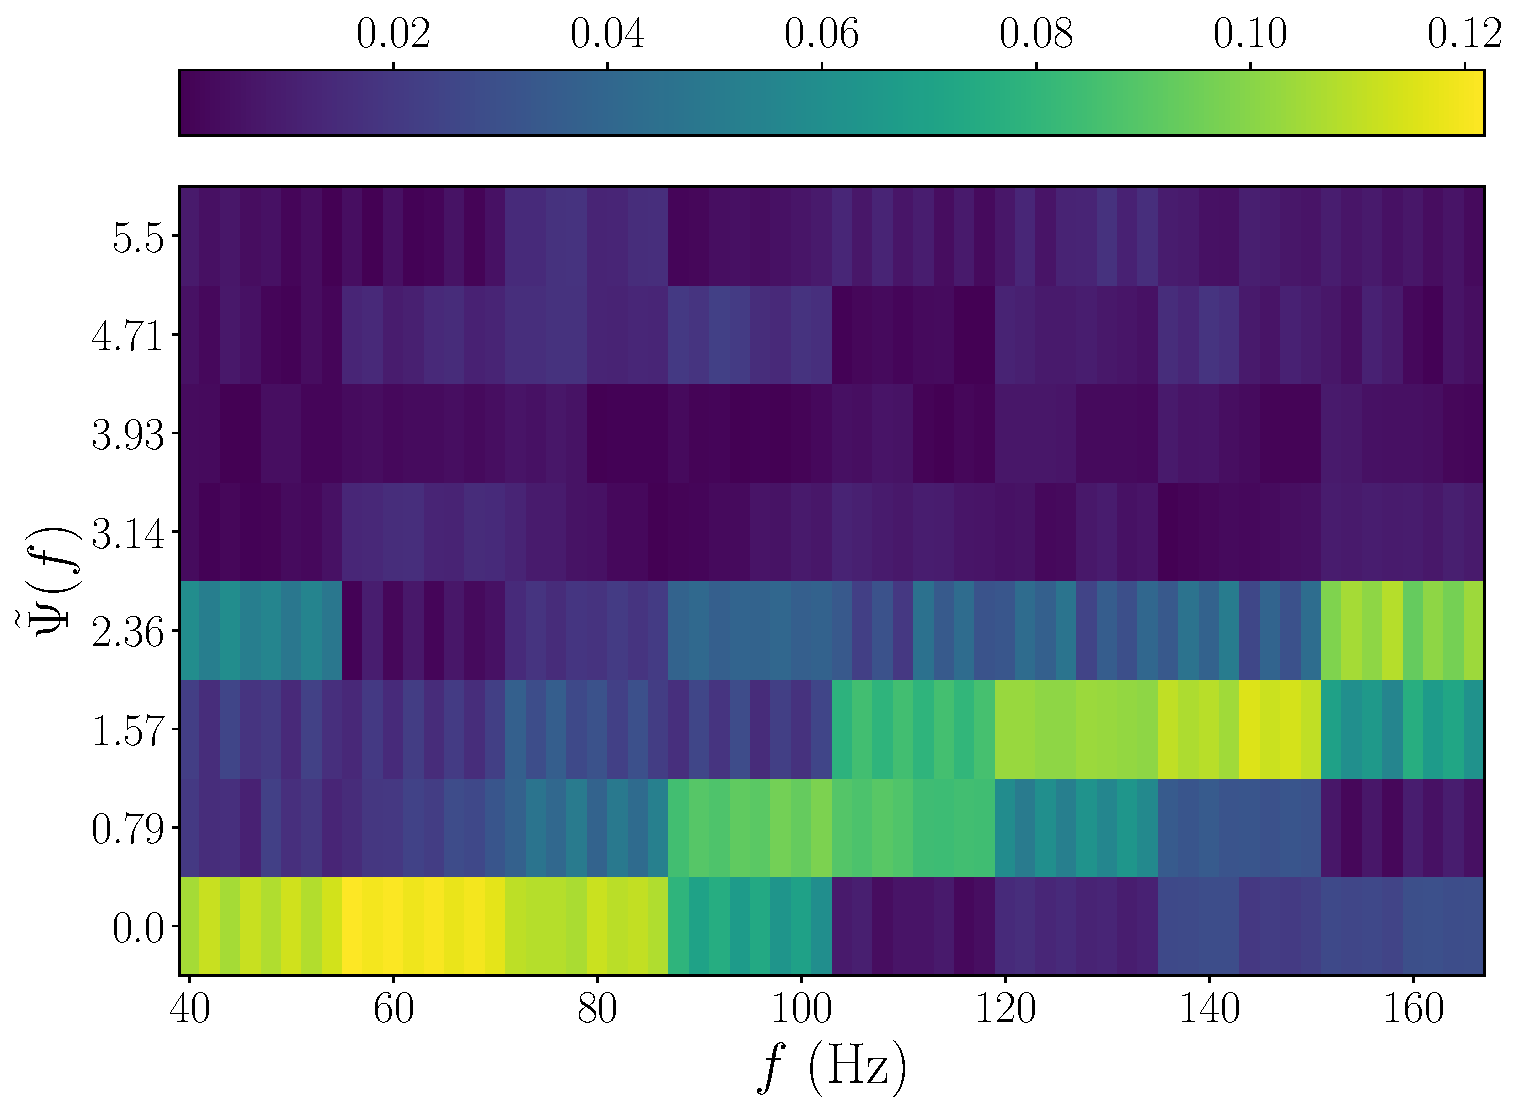
\includegraphics[width=\textwidth]{im/Q_amp_quadratic_0.6_H.pdf}
\caption{$\delta =0.6$}
\end{figure} 
\end{column}
\end{columns}
\end{frame}

\begin{frame}
\frametitle{Results}
Amplitudes after applying $\tilde{Q}$ with $\Psi(f) \sim f^2$ and the input register in initial state $\hat{H} \ket{0}$ ($L=\boldsymbol{9}$, $m=3$, SAM, 600 epochs):
\begin{columns}
\begin{column}{0.5\textwidth}
\begin{figure}
\centering
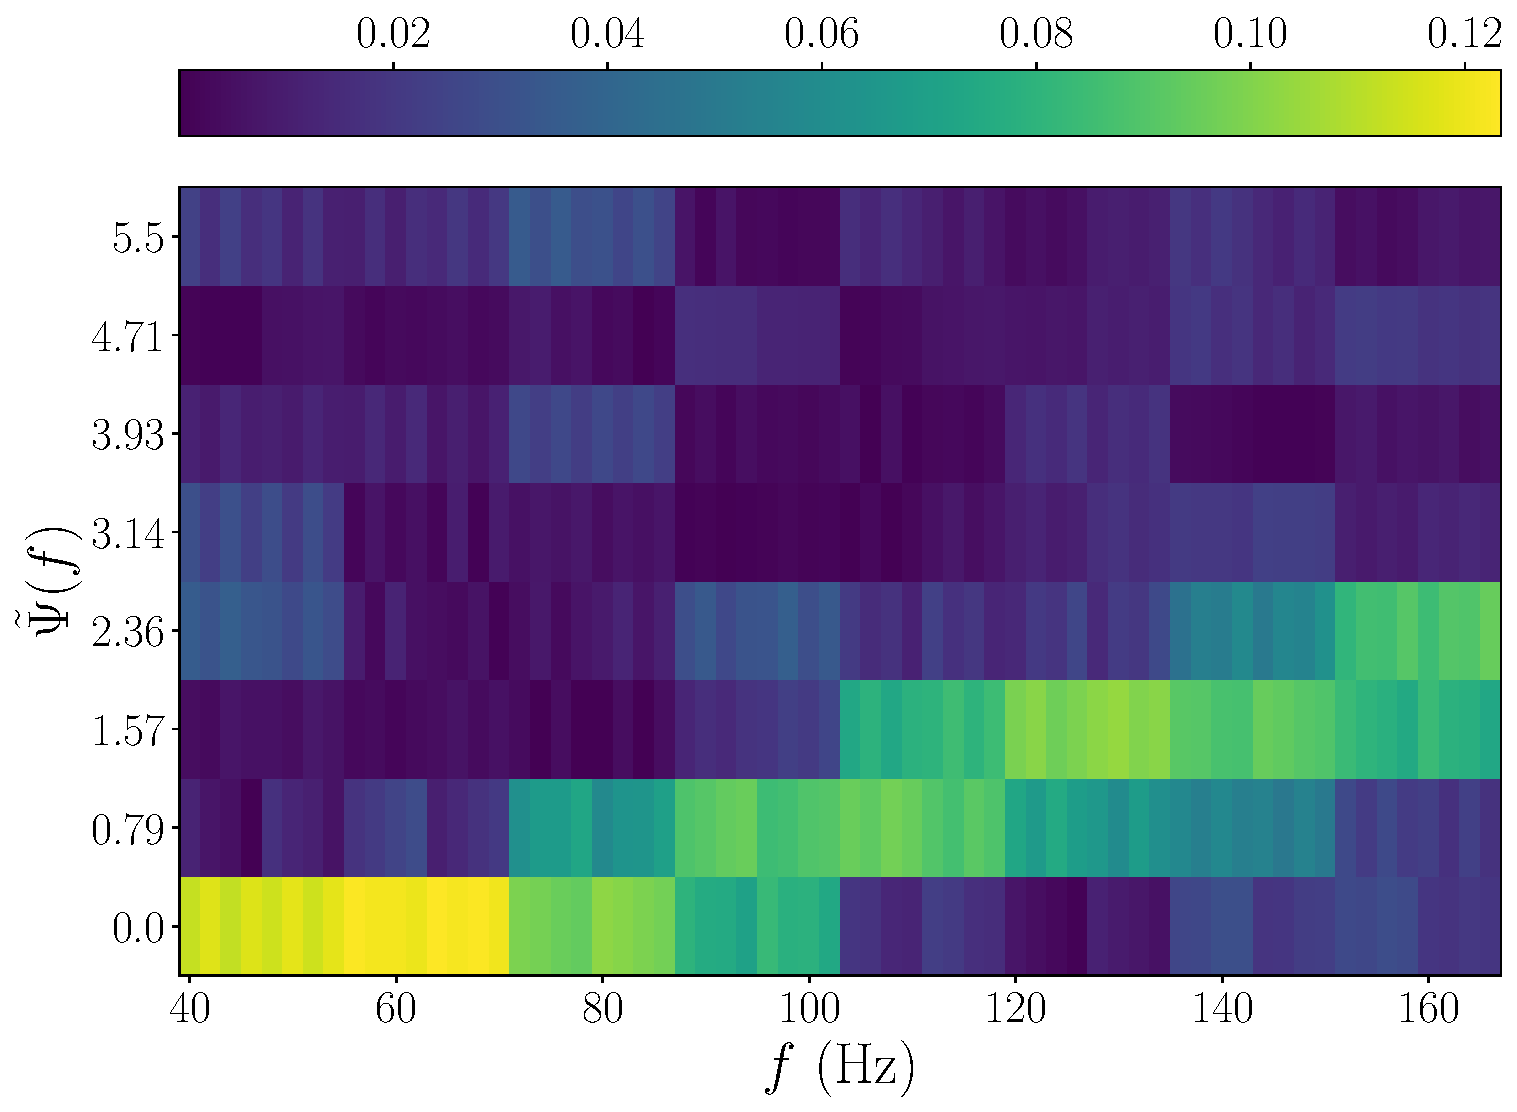
\includegraphics[width=\textwidth]{im/Q_amp_quadratic_0.8_H.pdf}
\caption{$\delta =0.8$}
\end{figure}
\end{column}
\begin{column}{0.5\textwidth}
\begin{figure}
\centering
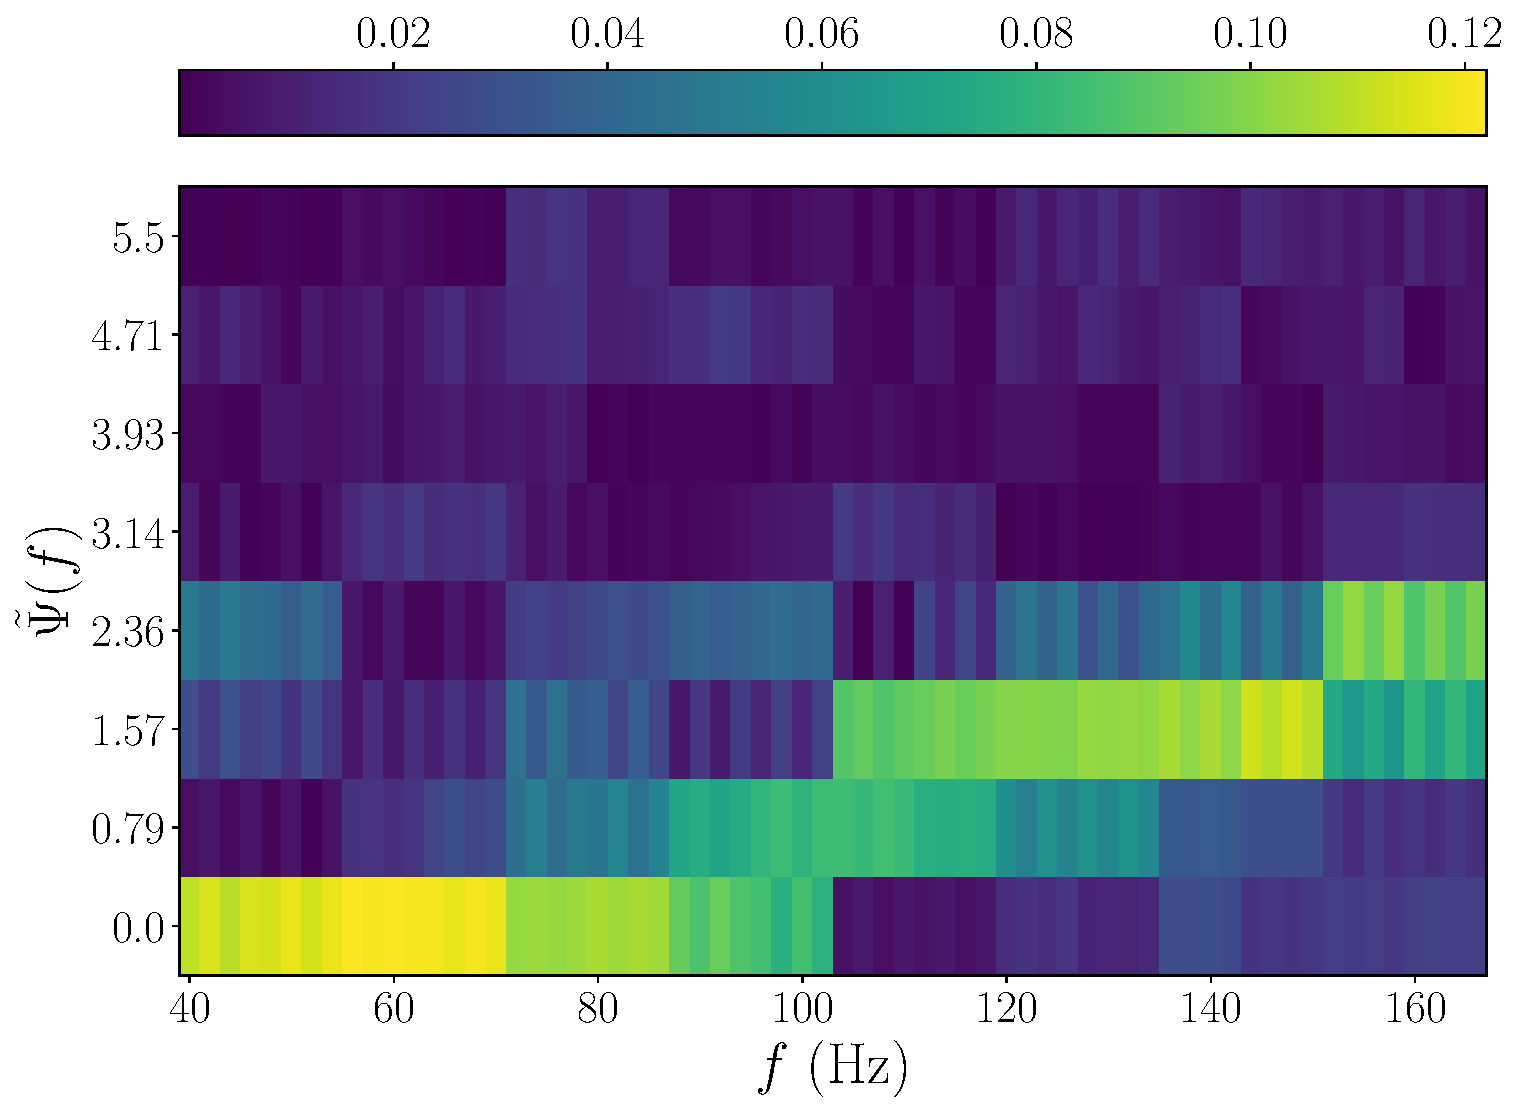
\includegraphics[width=\textwidth]{im/Q_amp_quadratic_1.0_H.pdf}
\caption{$\delta =1.0$}
\end{figure} 
\end{column}
\end{columns}
\end{frame}

\begin{frame}
\frametitle{Results}
\begin{columns}
\begin{column}{0.5\textwidth}
\begin{itemize}
\item Slightly randomised input states ($\delta = 0.2$)  have a \alert{positive effect} on performance
\item More significantly randomised input states ($\delta \geq 0.6$) have an \alert{adverse effect}
\item Notably, no positive effect of non-zero $\delta$ is apparent for $L=6$  
\item Also notable are the appearance of thin \alert{`stripes'} with increasing $\delta$ which could be linked to input layer structure
\item Equivalent effects are observed for $\Psi(f) \sim f $ and $\Psi_\text{H23}$
\end{itemize}
\end{column}
\begin{column}{0.5\textwidth}
\begin{figure}
\centering 
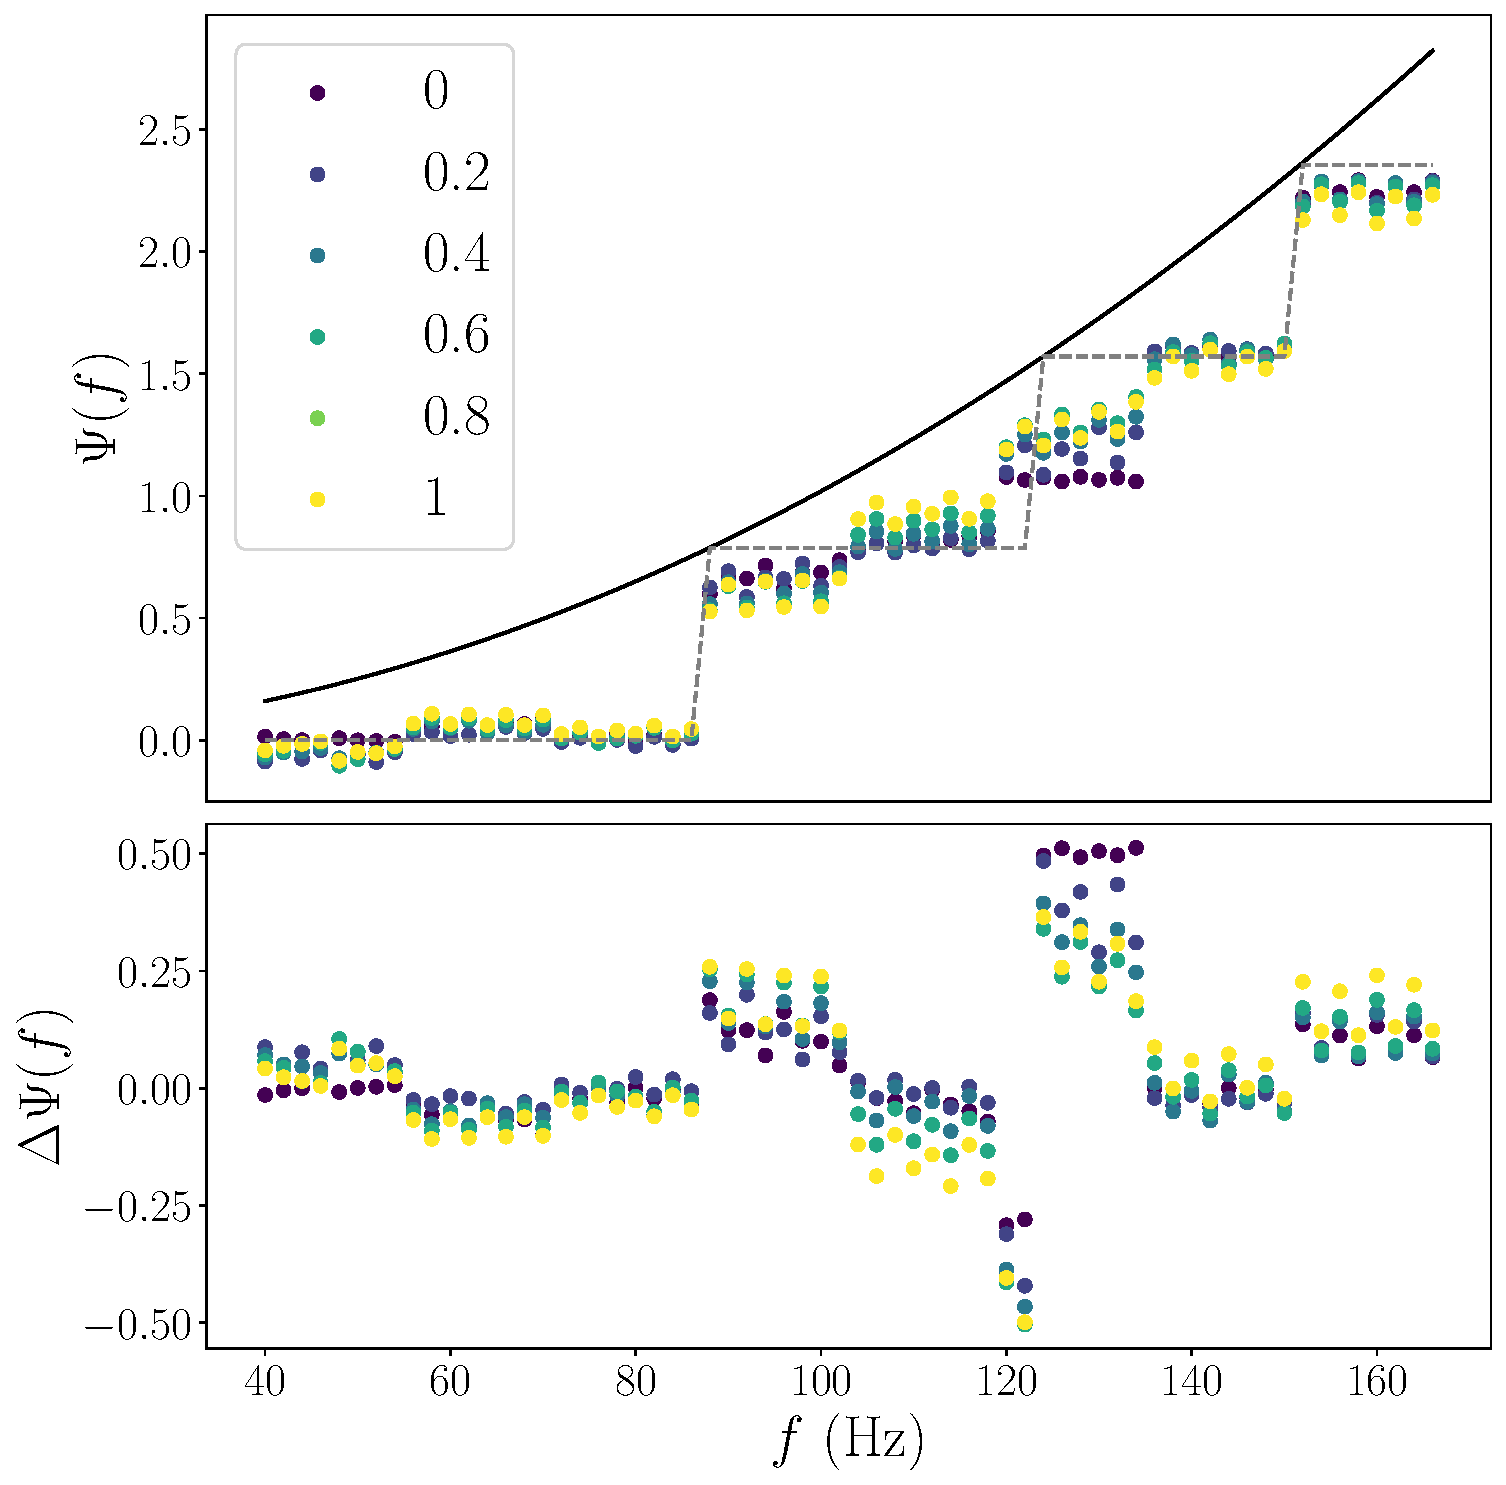
\includegraphics[width=\textwidth]{im/psi_comp_delta_L9}
\caption{Comparing the effect of $\delta$ values for $\Psi(f) \sim f^2$ ($L=9$, $m=3$, SAM, 600 epochs)}
\end{figure}
\end{column}
\end{columns}
\end{frame}

\begin{frame}
RUN THINGS FOR L=12 TO COMPARE !!


bug fix the benchmark plots, write docs strings, ...

SOMETHING WRONG WITH CALCULATING PHASE_TARGET_ROUNDED!!

then do more complex pltos 
\end{frame}

\section{Code and Documentation}

\begin{frame}
\frametitle{Code and Documentation}
\begin{itemize}
\item Continued work on code documentation: now hosted online \href{https://david-f-amorim.github.io/PQC_function_evaluation/pqcprep.html}{\textcolor{purple}{here}}
\end{itemize}
TO DO:
\begin{enumerate}[(a)]
\item write doc strings for testQNN, trainQNN, ampl\_trainQNN 
\item make sure to update doc files on github (-o /docs)
\item add plotting into comman-line feature (re-write plotting\_tools and check\_plots ...) 
\item integrate encode.py
\end{enumerate}
\end{frame}

\section{Next Steps}

\begin{frame}
\frametitle{Next Steps}

\begin{itemize}
\item Start work on poster for Carnegie 
\end{itemize}

\end{frame}

\end{document}